\documentclass{beamer}
\usepackage[utf8]{inputenc}
\usepackage{graphicx, epsfig}
\usepackage{amsmath,mathrsfs,amsfonts,amssymb}
%\usepackage{subfig}
\usepackage{floatflt}
\usepackage{epic,ecltree}
\usepackage{mathtext}
\usepackage{fancybox}
\usepackage{fancyhdr}
\usepackage{multirow}
\usepackage{enumerate}
\usepackage{epstopdf}
\usepackage{multicol}
\usepackage{algorithm}
\usepackage[noend]{algorithmic}
\usepackage{tikz}
\usepackage{blindtext}
\usetheme{default}%{Singapore}%{Warsaw}%{Warsaw}%{Darmstadt}
\usecolortheme{default}
\setbeamerfont{title}{size=\Huge}
\setbeamertemplate{footline}[page number]{}


\makeatletter
\newcommand\HUGE{\@setfontsize\Huge{35}{40}}
\makeatother    

\setbeamerfont{title}{size=\HUGE}
\beamertemplatenavigationsymbolsempty

% latin bold lower
\newcommand{\ba}{\mathbf{a}} 
\newcommand{\bc}{\mathbf{c}} 
\newcommand{\be}{\mathbf{e}} 
\newcommand{\bh}{\mathbf{h}} 
\newcommand{\bp}{\mathbf{p}} 
\newcommand{\bt}{\mathbf{t}} 
\newcommand{\bs}{\mathbf{s}} 
\newcommand{\bu}{\mathbf{u}} 
\newcommand{\bv}{\mathbf{v}} 
\newcommand{\bw}{\mathbf{w}} 
\newcommand{\bx}{\mathbf{x}} 
\newcommand{\by}{\mathbf{y}} 
\newcommand{\bz}{\mathbf{z}} 

% latin bold upper
\newcommand{\bA}{\mathbf{A}} 
\newcommand{\bB}{\mathbf{B}} 
\newcommand{\bC}{\mathbf{C}} 
\newcommand{\bI}{\mathbf{I}} 
\newcommand{\bL}{\mathbf{L}} 
\newcommand{\bM}{\mathbf{M}} 
\newcommand{\bQ}{\mathbf{Q}} 
\newcommand{\bT}{\mathbf{T}} 
\newcommand{\bU}{\mathbf{U}} 
\newcommand{\bV}{\mathbf{V}} 
\newcommand{\bW}{\mathbf{W}} 
\newcommand{\bX}{\mathbf{X}} 
\newcommand{\bY}{\mathbf{Y}} 
\newcommand{\bZ}{\mathbf{Z}} 

% latin cal upper
\newcommand{\cG}{\mathcal{G}} 
\newcommand{\cL}{\mathcal{L}} 
\newcommand{\cN}{\mathcal{N}} 
\newcommand{\cS}{\mathcal{S}} 
\newcommand{\cT}{\mathcal{T}} 
\newcommand{\cW}{\mathcal{W}} 
\newcommand{\cX}{\mathcal{X}} 
\newcommand{\cZ}{\mathcal{Z}} 

% latin bb upper
\newcommand{\bbE}{\mathbb{E}} 
\newcommand{\bbI}{\mathbb{I}} 
\newcommand{\bbP}{\mathbb{P}} 
\newcommand{\bbR}{\mathbb{R}} 

% greek bold lower
\newcommand{\bepsilon}{\boldsymbol{\epsilon}} 
\newcommand{\btheta}{\boldsymbol{\theta}} 
\newcommand{\blambda}{\boldsymbol{\lambda}} 
\newcommand{\bpi}{\boldsymbol{\pi}} 
\newcommand{\bmu}{\boldsymbol{\mu}} 
\newcommand{\bsigma}{\boldsymbol{\sigma}} 
\newcommand{\bphi}{\boldsymbol{\phi}} 

% greek bold upper
\newcommand{\bSigma}{\boldsymbol{\Sigma}} 

\DeclareMathOperator*{\argmin}{arg\,min}
\DeclareMathOperator*{\argmax}{arg\,max}

\newcommand{\createdgmtitle}[1]{\title[\hbox to 56mm{Deep Generative Models  \hfill\insertframenumber\,/\,\inserttotalframenumber}]
	{\vspace{1.5cm} \\ Deep Generative Models \\ {\Huge Lecture #1}}
	\author{Roman Isachenko}
	\institute{
	Moscow Institute of Physics and Technology
	} 
	\date{Autumn, 2021}
}

\newcommand\myfootnote[1]{%
  \tikz[remember picture,overlay]
  \draw (current page.south west) +(1in + \oddsidemargin,0.5em)
  node[anchor=south west,inner sep=0pt]{\parbox{\textwidth}{%
      \rlap{\rule{10em}{0.4pt}}\raggedright\scriptsize \textit{#1}}};}

\newcommand\myfootnotewithlink[2]{%
  \tikz[remember picture,overlay]
  \draw (current page.south west) +(1in + \oddsidemargin,0.5em)
  node[anchor=south west,inner sep=0pt]{\parbox{\textwidth}{%
      \rlap{\rule{10em}{0.4pt}}\raggedright\scriptsize\href{#1}{\textit{#2}}}};}
\createdgmtitle{7}
%--------------------------------------------------------------------------------
\begin{document}
%--------------------------------------------------------------------------------
\begin{frame}
%\thispagestyle{empty}
\titlepage
\end{frame}
%=======
\begin{frame}{Dequantization}
	\begin{itemize}
		\item Images are discrete data, pixels lie in the \{0, 255\} integer domain (the model is $P(\bx | \btheta) = \text{Categorical}(\bpi(\btheta))$).
		\item Flow is a continuous model (it works with continuous data $\bx$).
	\end{itemize}
	By fitting a continuous density model to discrete data, one can produce a degenerate solution with all probability mass on discrete values. \\
	How to convert a discrete data distribution to a continuous one?
	
	\begin{minipage}[t]{0.5\columnwidth}
		\begin{block}{Uniform dequantization}
		\vspace{-0.5cm}
			\begin{align*}
				\bx &\sim \text{Categorical}(\bpi) \\
				 \bu &\sim U[0, 1]
			\end{align*}
			\[
			\by = \bx + \bu \sim \text{Continuous} 
			\]
		\end{block}
	\end{minipage}%
	\begin{minipage}[t]{0.5\columnwidth}
		\begin{figure}
			\centering
			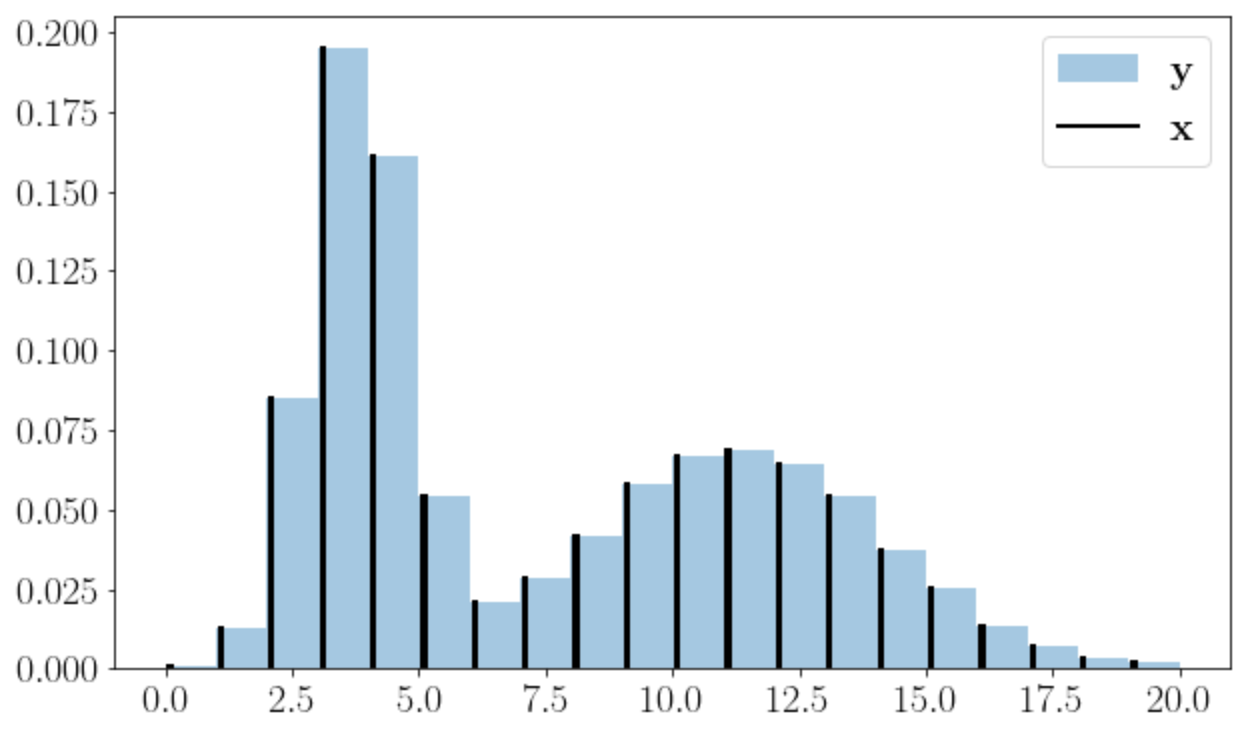
\includegraphics[width=1.0\linewidth]{figs/uniform_dequantization.png}
		\end{figure}
	\end{minipage}
	\myfootnotewithlink{https://arxiv.org/abs/1511.01844}{Theis L., Oord A., Bethge M. A note on the evaluation of generative models. 2015}
\end{frame}
%=======
\begin{frame}{Uniform dequantization}
	\begin{block}{Statement}
		Fitting continuous model $p(\by | \btheta)$ on uniformly dequantized data $\by = \bx + \bu, \, \bu \sim U[0, 1]$ is equivalent to maximization of a lower bound on log-likelihood for a discrete model:
		\vspace{-0.2cm}
		\[
		P(\bx | \btheta) = \int_{U[0, 1]} p(\bx + \bu | \btheta) d \bu
		\]
		\vspace{-0.5cm} 
	\end{block}
	\begin{block}{Proof}
		\vspace{-0.8cm}
		\begin{multline*}
			\bbE_{\pi} \log p(\by | \btheta) = \int \pi(\by) \log p(\by | \btheta) d \by = \\ 
			= \sum \pi(\bx) \int_{U[0,1]} \log p(\bx + \bu | \btheta) d \bu \leq \\
			 \leq \sum \pi(\bx) \log \int_{U[0,1]}  p(\bx + \bu | \btheta) d \bu = \\
			 = \sum \pi(\bx) \log P(\bx | \btheta) = \bbE_{\pi} \log P(\bx | \btheta).
		\end{multline*}
	\end{block}
	\myfootnotewithlink{https://arxiv.org/abs/1511.01844}{Theis L., Oord A., Bethge M. A note on the evaluation of generative models. 2015}
\end{frame}
%=======
\begin{frame}{Variational dequantization}
	\begin{minipage}[t]{0.5\columnwidth}
			\begin{figure}
				\centering
				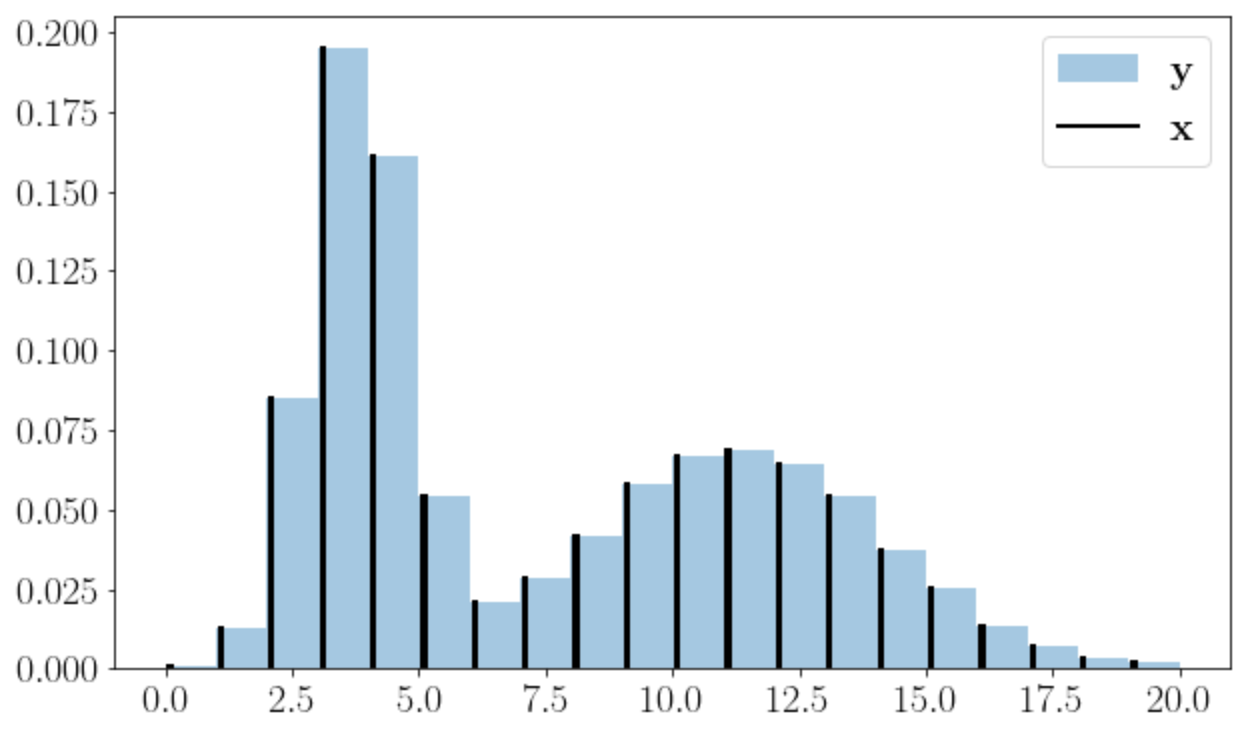
\includegraphics[width=1.0\linewidth]{figs/uniform_dequantization.png}
			\end{figure}
	\end{minipage}%
	\begin{minipage}[t]{0.5\columnwidth}
		\begin{figure}
			\centering
			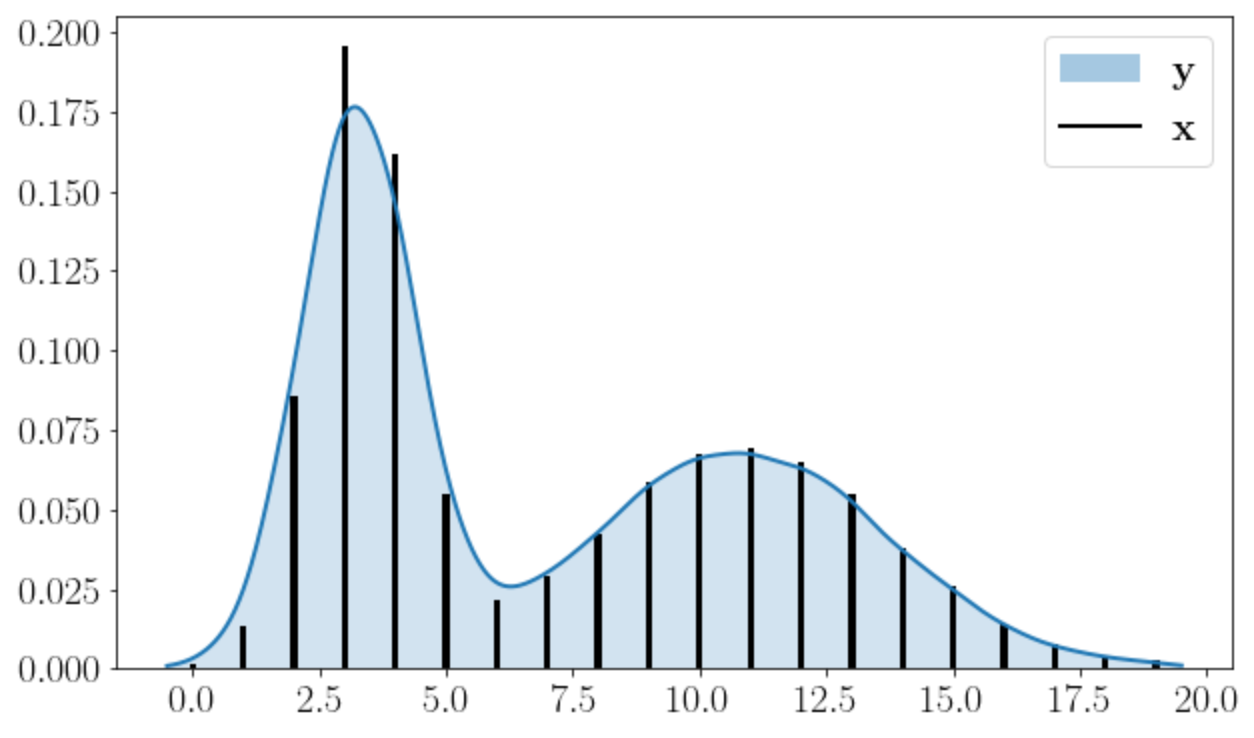
\includegraphics[width=1.0\linewidth]{figs/variational_dequantization.png}
		\end{figure}
	\end{minipage}
	\begin{itemize}
		\item $p(\by | \btheta)$ assign unifrom density to unit hypercubes $\bx + U[0, 1]$ (left fig).
		\item Neural network density models are smooth function approximators (right fig).
		\item Smooth dequantization is more natural.
	\end{itemize}
	How to perform the smooth dequantization? \\
\end{frame}
%=======
\begin{frame}{Flow++}
	\begin{block}{Variational dequantization}
		Introduce variational dequantization noise distribution $q(\bu | \bx)$ and treat it as an approximate posterior. 
	\end{block}
	\begin{block}{Variational lower bound}
		\vspace{-0.7cm}
		\begin{multline*}
		 \log P(\bx | \btheta) = \left[ \log \int q(\bu | \bx) \frac{p(\bx + \bu | \btheta)}{q(\bu | \bx)} d \bu \right] \geq \\ 
			\geq  \int q(\bu | \bx) \log \frac{p(\bx + \bu | \btheta)}{q(\bu | \bx)} d \bu = \mathcal{L}(q, \btheta).
		\end{multline*}
	\end{block}
	\vspace{-0.5cm}
	\begin{block}{Uniform dequantization bound}
		\vspace{-0.4cm}
		\[
		 \log P(\bx | \btheta) = \log \int_{U[0, 1]} p(\bx + \bu | \btheta) d \bu \geq \int_{U[0, 1]} \log p(\bx + \bu | \btheta) d \bu.
		\]
	\end{block}
	\myfootnotewithlink{https://arxiv.org/abs/1902.00275}{Ho J. et al. Flow++: Improving Flow-Based Generative Models with Variational Dequantization and Architecture Design, 2019}
\end{frame}
%=======
\begin{frame}{Flow++}
	\begin{block}{Variational lower bound}
		\[
		\mathcal{L}(q, \btheta) = \int q(\bu | \bx) \log \frac{p(\bx + \bu | \btheta)}{q(\bu | \bx)} d \bu.
		\]
	\end{block}
	Let $\bu = h(\bepsilon, \bphi)$ is a flow model with base distribution $\bepsilon \sim p(\bepsilon) = \mathcal{N}(0, \mathbf{I})$:
	\vspace{-0.3cm}
	\[
		q(\bu | \bx) = p(h^{-1}(\bu, \bphi)) \cdot \left| \det \frac{\partial h^{-1}(\bu, \bphi)}{\partial \bu}\right|.
	\]
	\vspace{-0.3cm}
	Then
	\[
		\log P(\bx | \btheta) \geq \cL(\bphi, \btheta) = \int p(\bepsilon) \log \left( \frac{p(\bx + h(\bepsilon, \bphi) | \btheta)}{p(\bepsilon) \cdot \left| \det \frac{\partial h(\bepsilon, \bphi)}{\partial \bepsilon}\right|^{-1}} \right) d\bepsilon.
	\]
	\myfootnotewithlink{https://arxiv.org/abs/1902.00275}{Ho J. et al. Flow++: Improving Flow-Based Generative Models with Variational Dequantization and Architecture Design, 2019}
\end{frame}
%=======
\begin{frame}{Flow++}
	\begin{block}{Variational lower}
	\vspace{-0.3cm}
	\[
		\log P(\bx | \btheta) \geq \int p(\bepsilon)\log \left( \frac{p(\bx + h(\bepsilon, \bphi))}{p(\bepsilon) \cdot \left| \det \frac{\partial h(\bepsilon, \bphi)}{\partial \bepsilon}\right|^{-1}} \right) d\bepsilon.
	\]
	\end{block}
	\begin{itemize}
	\item If $p(\bx + \bu | \btheta)$ is also a flow model, it is straightforward to calculate stochastic gradient of this ELBO.
	
	\item Uniform dequantization is a special case of variational dequantization ($q(\bu | \bx) = U[0, 1]$).
	The gap between $\log P(\bx | \btheta)$ and the derived ELBO is 
	$ KL(q(\bu | \bx) || p(\bu | \bx))$.
	\item In the case of uniform dequantization the model unnaturally places uniform density over each hypercube $\bx + U[0, 1]$ due to inexpressive distribution $q$.
	\end{itemize}
	\myfootnotewithlink{https://arxiv.org/abs/1902.00275}{Ho J. et al. Flow++: Improving Flow-Based Generative Models with Variational Dequantization and Architecture Design, 2019}
\end{frame}
%=======
\begin{frame}{Flow++}
	\begin{figure}
		\centering
		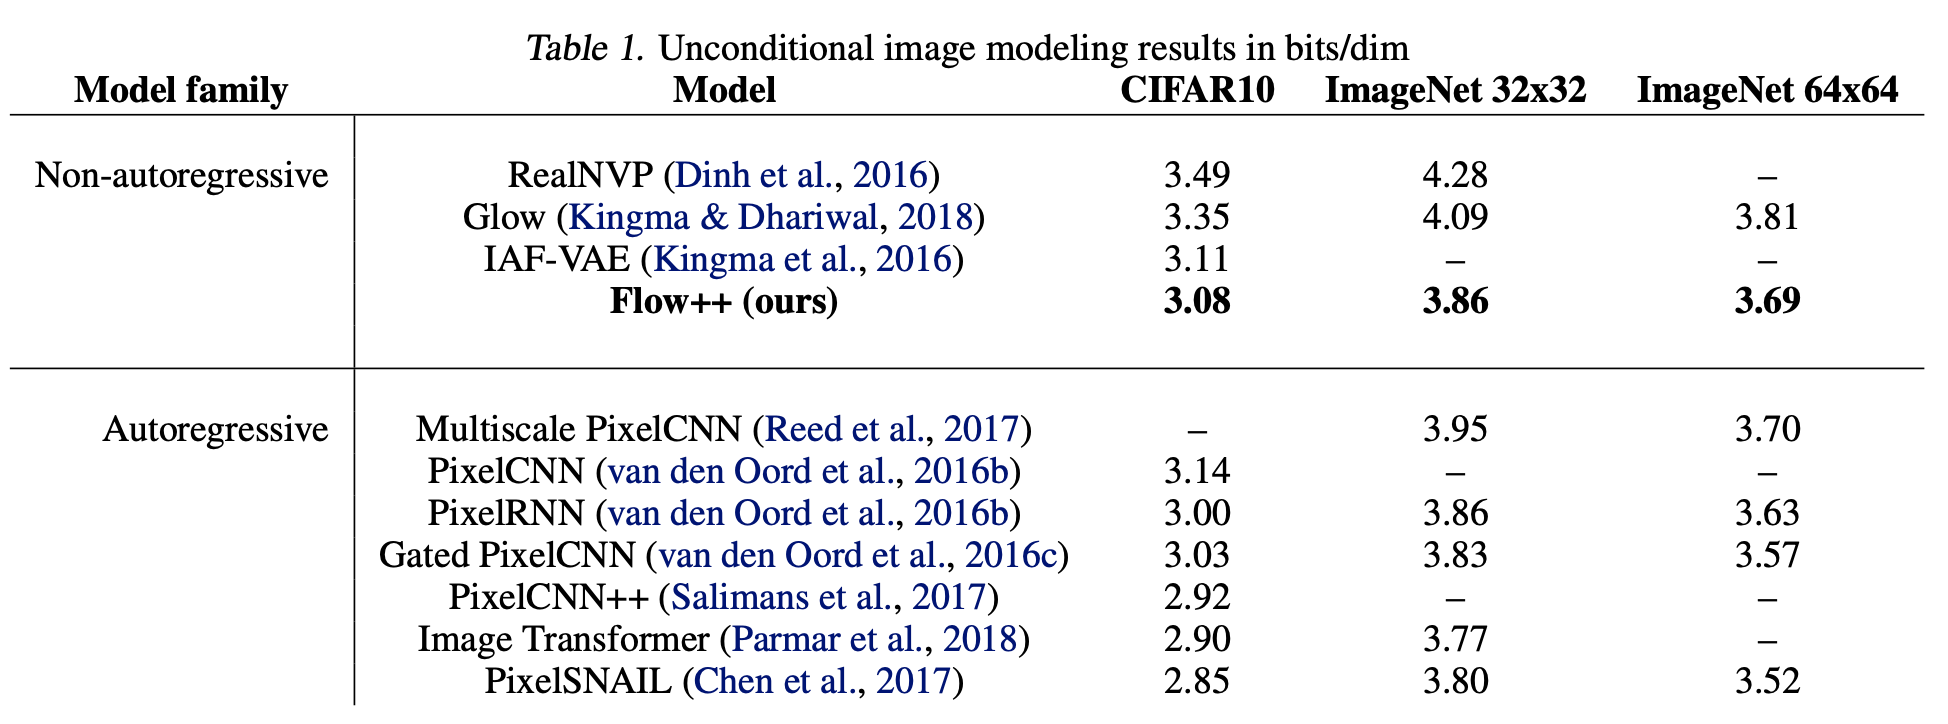
\includegraphics[width=0.7\linewidth]{figs/flow++1.png}
	\end{figure}
	\vspace{-0.1cm}
	\begin{figure}
		\centering
		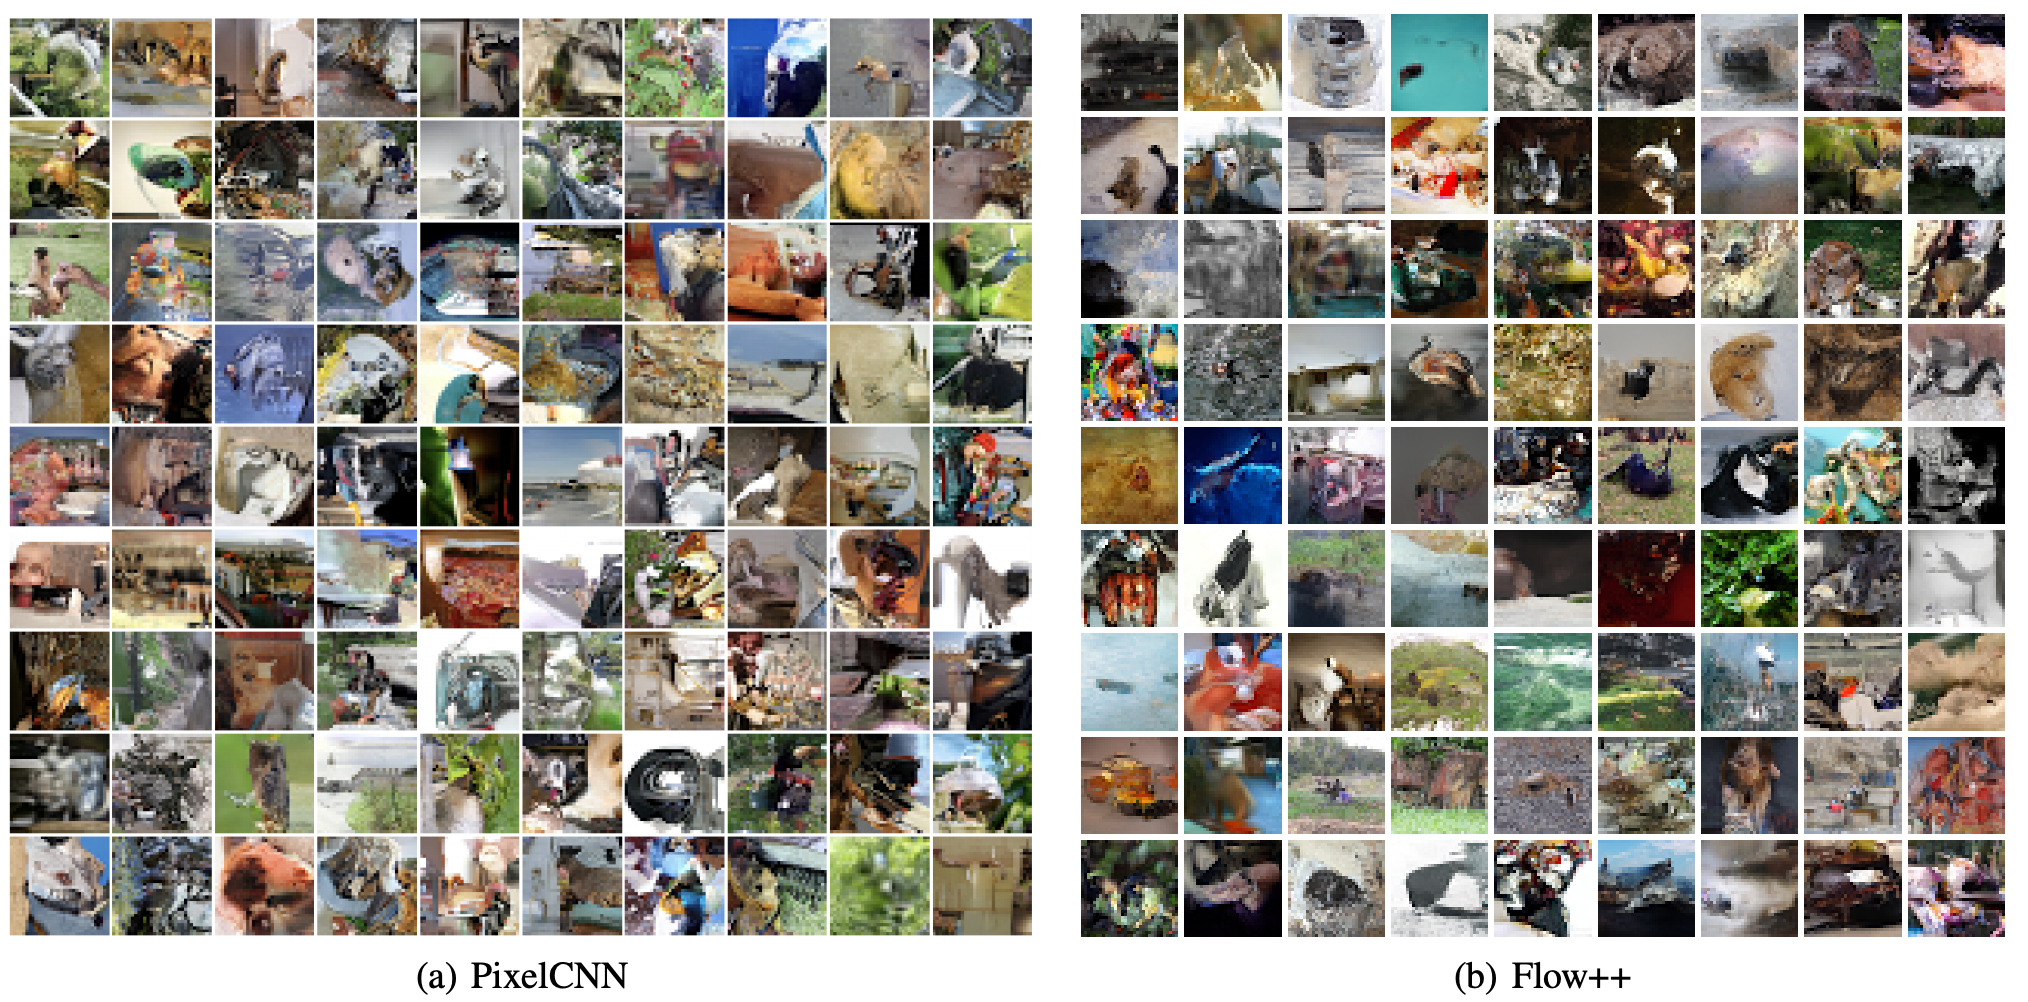
\includegraphics[width=0.8\linewidth]{figs/flow++2.png}
	\end{figure}
	\myfootnotewithlink{https://arxiv.org/abs/1902.00275}{Ho J. et al. Flow++: Improving Flow-Based Generative Models with Variational Dequantization and Architecture Design, 2019}
\end{frame}
%=======
\begin{frame}{VAE limitations}
	\begin{itemize}
		\item Poor variational posterior distribution (encoder)
		\[
		q(\bz | \bx, \bphi) = \mathcal{N}(\bz| \bmu_{\bphi}(\bx), \bsigma^2_{\bphi}(\bx)).
		\]
		\item Poor prior distribution
		\[
		p(\bz) = \mathcal{N}(0, \mathbf{I}).
		\]
		\item Poor probabilistic model (decoder)
		\[
		p(\bx | \bz, \btheta) = \mathcal{N}(\bx| \bmu_{\btheta}(\bz), \bsigma^2_{\btheta}(\bz)).
		\]
		\item Loose lower bound
		\[
		\log p(\bx | \btheta) - \mathcal{L}(q, \btheta) = (?).
		\]
	\end{itemize}
\end{frame}
%=======
\begin{frame}{Importance Sampling}
	\begin{block}{Generative model}
		\vspace{-0.5cm}
		\begin{align*}
			p(\bx | \btheta) &= \int p(\bx, \bz | \btheta) d\bz = \int \left[\frac{p(\bx, \bz | \btheta)}{q(\bz | \bx)} \right] q(\bz | \bx) d\bz \\
			&= \int f(\bx, \bz) q(\bz | \bx) d\bz = \mathbb{E}_{\bz \sim q(\bz | \bx)} f(\bx, \bz)
		\end{align*}
	\end{block}
	Here $f(\bx, \bz) = \frac{p(\bx, \bz | \btheta)}{q(\bz | \bx)}$.
	\begin{block}{ELBO}
		\vspace{-0.5cm}
		\begin{multline*}
			\log p(\bx | \btheta) = \log \mathbb{E}_{\bz \sim q(\bz | \bx)} f(\bx, \bz)
			\geq \mathbb{E}_{\bz \sim q(\bz | \bx)} \log f(\bx, \bz) = \\
			= \mathbb{E}_{\bz \sim q(\bz | \bx)} \log \frac{p(\bx, \bz | \btheta)}{q(\bz | \bx)} = \mathcal{L}(q, \btheta).
		\end{multline*}
	\end{block}
	Could we choose better $f(\bx, \bz)$? 
\end{frame}
%=======
\begin{frame}{IWAE}
		\[
			p(\bx | \btheta) = \int p(\bx, \bz | \btheta) d\bz = \int \left[\frac{p(\bx, \bz | \btheta)}{q(\bz | \bx)} \right] q(\bz | \bx) d\bz = \mathbb{E}_{\bz \sim q(\bz | \bx)} f(\bx, \bz)
		\]
	Let define
	\[
	f(\bx, \bz_1, \dots, \bz_K) = \frac{1}{K} \sum_{k=1}^K \frac{p(\bx, \bz_k | \btheta)}{q(\bz_k | \bx)}
	\]
	\[
		\mathbb{E}_{\bz_1, \dots, \bz_K \sim q(\bz | \bx)} f(\bx, \bz_1, \dots, \bz_K) = p(\bx | \btheta)
	\]
	\vspace{-0.3cm}
	\begin{block}{ELBO}
		\vspace{-0.5cm}
		\begin{multline*}
			\log p(\bx | \btheta) = \log \mathbb{E}_{\bz_1, \dots, \bz_K \sim q(\bz | \bx)} f(\bx, \bz, \dots, \bz_K) \geq \\
			\geq \mathbb{E}_{\bz_1, \dots, \bz_K \sim q(\bz | \bx)} \log f(\bx, \bz, \dots, \bz_K) = \\
			= \mathbb{E}_{\bz_1, \dots, \bz_K \sim q(\bz | \bx)} \log \left[\frac{1}{K} \sum_{k=1}^K\frac{p(\bx, \bz_k | \btheta)}{q(\bz_k | \bx)} \right] = \mathcal{L}_K(q, \btheta).
		\end{multline*}
	\end{block}
	\myfootnotewithlink{https://arxiv.org/abs/1509.00519}{Burda Y., Grosse R., Salakhutdinov R. Importance Weighted Autoencoders, 2015}
\end{frame}
%=======
\begin{frame}{IWAE}
	\begin{block}{VAE objective}
		\vspace{-0.2cm}
		\[
		\log p(\bx | \btheta) \geq \mathcal{L} (q, \btheta)  = \mathbb{E}_{q(\bz | \bx)} \log \frac{p(\bx, \bz | \btheta)}{q(\bz| \bx)} \rightarrow \max_{q, \btheta}
		\]
		\[
		\mathcal{L} (q, \btheta)  = \mathbb{E}_{\bz_1, \dots, \bz_K \sim q(\bz | \bx)} \left( \frac{1}{K} \sum_{k=1}^K \log \frac{p(\bx, \bz_k | \btheta)}{q(\bz_k| \bx)} \right) \rightarrow \max_{q, \btheta}.
		\]
		\vspace{-0.2cm}
	\end{block}
	\begin{block}{IWAE objective}
		\vspace{-0.2cm}
		\[
		\mathcal{L}_K (q, \btheta)  = \mathbb{E}_{\bz_1, \dots, \bz_K \sim q(\bz | \bx)} \log \left( \frac{1}{K}\sum_{k=1}^K\frac{p(\bx, \bz_k | \btheta)}{q(\bz_k| \bx)} \right) \rightarrow \max_{q, \btheta}.
		\]
	\end{block}
	If $K=1$, these objectives coincide.

	\myfootnotewithlink{https://arxiv.org/abs/1509.00519}{Burda Y., Grosse R., Salakhutdinov R. Importance Weighted Autoencoders, 2015}
\end{frame}
%=======
\begin{frame}{IWAE}
	\begin{block}{Theorem}
		\begin{enumerate}
			\item $\log p(\bx | \btheta) \geq \mathcal{L}_K (q, \btheta) \geq \mathcal{L}_M (q, \btheta), \quad \text{for } K \geq M$;
			\item $\log p(\bx | \btheta) = \lim_{K \rightarrow \infty} \mathcal{L}_K (q, \btheta)$ if $\frac{p(\bx, \bz | \btheta)}{q(\bz | \bx)}$ is bounded.
		\end{enumerate}
		\vspace{-0.2cm}
	\end{block}
	\begin{block}{Proof of 1.}
		{ \footnotesize
			\vspace{-0.5cm}
			\begin{align*}
				\mathcal{L}_K (q, \btheta) &= \mathbb{E}_{\bz_1, \dots, \bz_K} \log \left( \frac{1}{K}\sum_{k=1}^K\frac{p(\bx, \bz_k | \btheta)}{q(\bz_k| \bx)} \right) = \\
				&= \mathbb{E}_{\bz_1, \dots, \bz_K} \log \mathbb{E}_{k_1, \dots, k_M} \left( \frac{1}{M}\sum_{m=1}^M\frac{p(\bx, \bz_{k_m} | \btheta)}{q(\bz_{k_m}| \bx)} \right) \geq \\
				&\geq \mathbb{E}_{\bz_1, \dots, \bz_K} \mathbb{E}_{k_1, \dots, k_m} \log \left( \frac{1}{M}\sum_{m=1}^M\frac{p(\bx, \bz_{k_m} | \btheta)}{q(\bz_{k_m}| \bx)} \right) = \\
				&= \mathbb{E}_{\bz_1, \dots, \bz_M} \log \left( \frac{1}{M}\sum_{m=1}^M\frac{p(\bx, \bz_m | \btheta)}{q(\bz_m| \bx)} \right) = \mathcal{L}_M (q, \btheta)
			\end{align*}
			\[
			\frac{a_1 + \dots + a_K}{K} = \mathbb{E}_{k_1, \dots, k_M} \frac{a_{k_1} + \dots + a_{k_M}}{M}, \quad k_1, \dots, k_M \sim U[1, K]
			\]
		}
	\end{block}
	
	\myfootnotewithlink{https://arxiv.org/abs/1509.00519}{Burda Y., Grosse R., Salakhutdinov R. Importance Weighted Autoencoders, 2015}
\end{frame}
%=======
\begin{frame}{IWAE}
	\begin{block}{Theorem}
		\begin{enumerate}
			\item $\log p(\bx | \btheta) \geq \mathcal{L}_K (q, \btheta) \geq \mathcal{L}_M (q, \btheta), \quad \text{for} K \geq M$;
			\item $\log p(\bx | \btheta) = \lim_{K \rightarrow \infty} \mathcal{L}_K (q, \btheta)$ if $\frac{p(\bx, \bz | \btheta)}{q(\bz | \bx)}$ is bounded.
		\end{enumerate}
		\vspace{-0.2cm}
	\end{block}
	\begin{block}{Proof of 2.}
		\vspace{0.2cm}
		Consider r.v. $\xi_K = \frac{1}{K}\sum_{k=1}^K \frac{p(\bx, \bz_k | \btheta)}{q(\bz_k | \bx)}$. \\
		\vspace{0.2cm}
		If summands are bounded, then (from the strong law of large numbers)
		\[
		\xi_K \xrightarrow[K \rightarrow \infty]{a.s.} \mathbb{E}_{q(\bz | \bx)} \frac{p(\bx, \bz | \btheta)}{q(\bz | \bx)} = p(\bx | \btheta).
		\]
		Hence $\mathcal{L}_K (q, \btheta) = \mathbb{E} \log \xi_K$ converges to $\log p(\bx | \btheta)$ as $K \rightarrow \infty$.
	\end{block}

	\myfootnotewithlink{https://arxiv.org/abs/1509.00519}{Burda Y., Grosse R., Salakhutdinov R. Importance Weighted Autoencoders, 2015}
\end{frame}
%=======
\begin{frame}{IWAE}
	\[
	\log p(\bx | \btheta) \geq \mathcal{L}_K(q, \btheta) \geq \mathcal{L}(q, \btheta)
	\]
	If $K > 1$ the bound could be tighter.
	\begin{align*}
		\mathcal{L} (q, \btheta) &= \mathbb{E}_{q(\bz | \bx)} \log \frac{p(\bx, \bz | \btheta)}{q(\bz| \bx)}; \\
		\mathcal{L}_K (q, \btheta) &= \mathbb{E}_{\bz_1, \dots, \bz_K \sim q(\bz | \bx)} \log \left( \frac{1}{K}\sum_{k=1}^K\frac{p(\bx, \bz_k | \btheta)}{q(\bz_k| \bx)} \right).
	\end{align*}
	\vspace{-0.2cm}
	\begin{itemize}
		\item $\mathcal{L}_1(q, \btheta) = \mathcal{L}(q, \btheta)$;
		\item $\mathcal{L}_{\infty}(q, \btheta) = \log p(\bx | \btheta)$.
		\item Which $q^*(\bz | \bx)$ gives $\mathcal{L}(q^*, \btheta) = \log p(\bx | \btheta)$? 
		\item Which $q^*(\bz | \bx)$ gives $\mathcal{L}(q^*, \btheta) = \mathcal{L}_K(q, \btheta)$?
	\end{itemize}

	\myfootnotewithlink{https://arxiv.org/abs/1509.00519}{Burda Y., Grosse R., Salakhutdinov R. Importance Weighted Autoencoders, 2015}
\end{frame}
%=======
\begin{frame}{IWAE}
	\begin{block}{Theorem}
		The VAE objective is equal to IWAE objective 
		\[
		\mathcal{L}(q_{EW}, \btheta) = \mathcal{L}_K(q, \btheta)
		\]
		for the following variational distribution
		\[
		q_{EW}(\bz | \bx) = \mathbb{E}_{\bz_2, \dots, \bz_K \sim q(\bz | \bx)} q_{IW}(\bz | \bx, \bz_{2:K}),
		\]
		where \[
		q_{IW}(\bz | \bx, \bz_{2:K}) = \frac{\frac{p(\bx, \bz)}{q(\bz | \bx)}}{\frac{1}{K} \sum_{k=1}^K \frac{p(\bx, \bz_k)}{q(\bz_k | \bx)}} q(\bz | \bx) = \frac{p(\bx, \bz)}{\frac{1}{K}\left( \frac{p(\bx, \bz)}{q(\bz | \bx)} + \sum_{k=2}^K \frac{p(\bx, \bz_k)}{q(\bz_k | \bx)}\right)}.
		\]
	\end{block}
	
	\myfootnotewithlink{https://arxiv.org/abs/1704.02916}{Cremer C., Morris Q., Duvenaud D. Reinterpreting Importance-Weighted Autoencoders, 2017}
\end{frame}
%=======
\begin{frame}{IWAE}
	\begin{block}{IWAE posterior}
		\vspace{-0.3cm}
		\begin{figure}
			\centering
			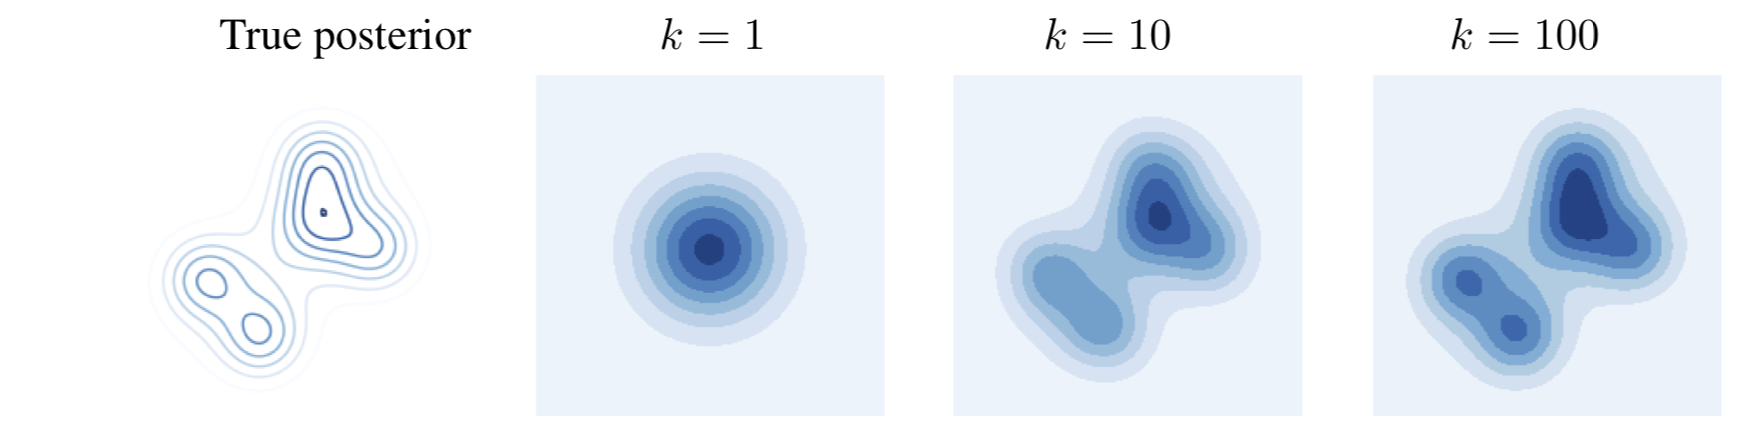
\includegraphics[width=\linewidth]{figs/IWAE_1.png}
		\end{figure}
	\end{block}
	\vspace{-0.5cm}
	\begin{block}{IWAE samples}
		\vspace{-0.3cm}
		\begin{figure}
			\centering
			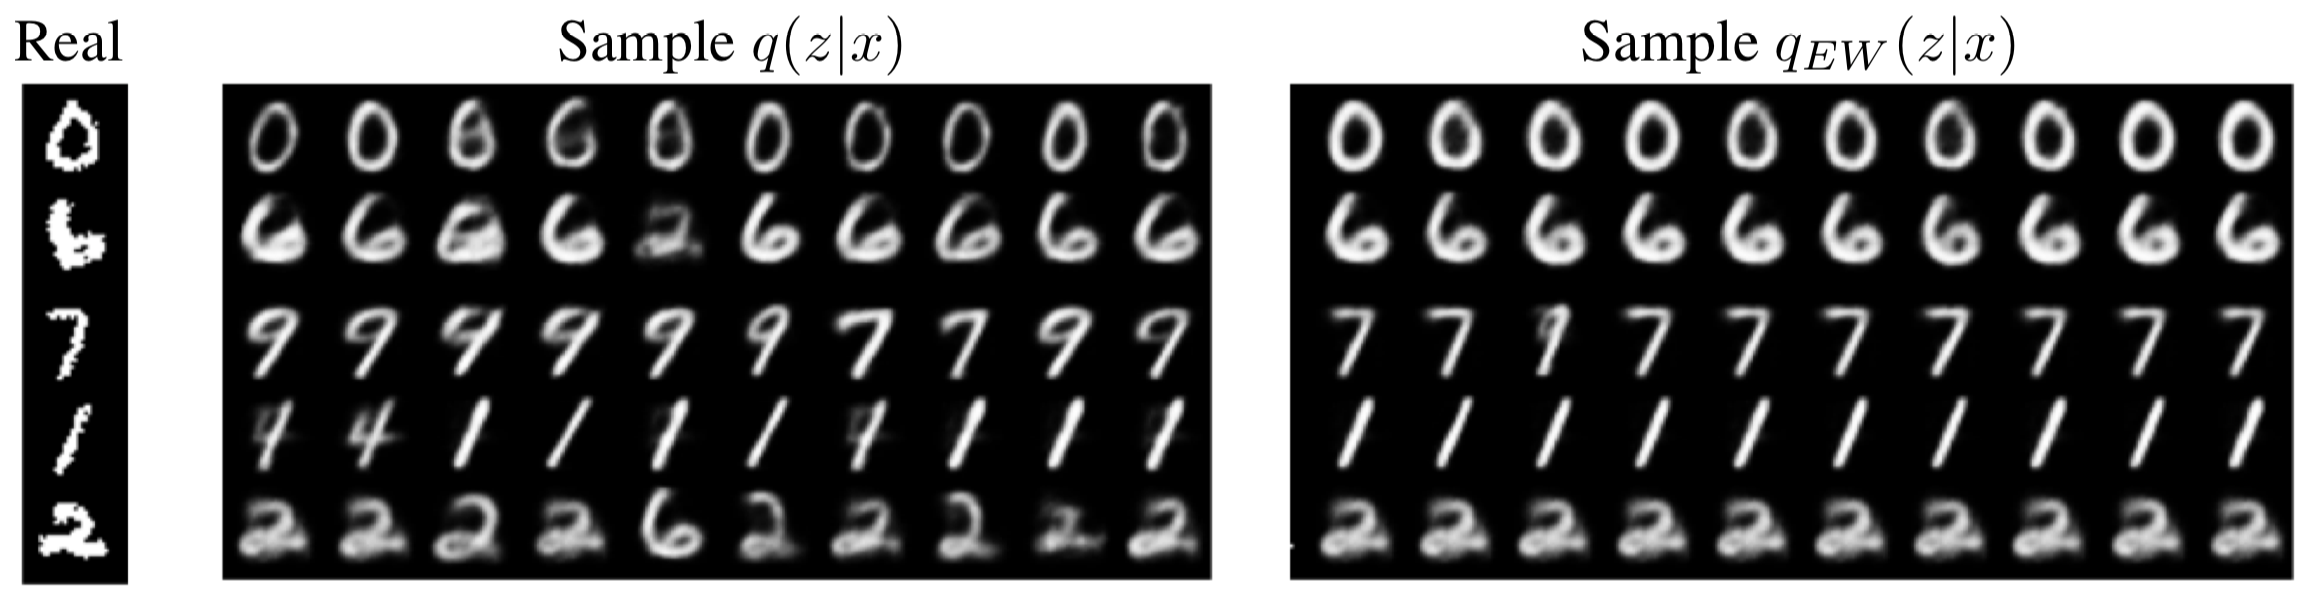
\includegraphics[width=\linewidth]{figs/IWAE_2.png}
		\end{figure}
	\end{block}

	\myfootnotewithlink{https://arxiv.org/abs/1704.02916}{Cremer C., Morris Q., Duvenaud D. Reinterpreting Importance-Weighted Autoencoders, 2017}
\end{frame}
%=======
\begin{frame}{IWAE}
	\begin{block}{Objective}
		\vspace{-0.5cm}
		\[
		\mathcal{L}_K (q, \btheta)  = \mathbb{E}_{\bz_1, \dots, \bz_K \sim q(\bz | \bx, \bphi)} \log \left( \frac{1}{K}\sum_{k=1}^K\frac{p(\bx, \bz_k | \btheta)}{q(\bz_k| \bx, \bphi)} \right) \rightarrow \max_{\bphi, \btheta}.
		\]
		\vspace{-0.3cm}
	\end{block}
	\begin{block}{Gradient}
		\vspace{-0.3cm}
		\[
		\Delta_K = \nabla_{\btheta, \bphi} \log \left( \frac{1}{K}\sum_{k=1}^K\frac{p(\bx, \bz_k | \btheta)}{q(\bz_k| \bx, \bphi)} \right), \quad \bz_k \sim q(\bz | \bx, \bphi).
		\]
		\vspace{-0.3cm}
	\end{block}
	\begin{block}{Theorem}
		\vspace{-0.4cm}
		\[
			\text{SNR}_K = \frac{\bbE [\Delta_K]}{\sigma(\Delta_K)}; \quad
			\text{SNR}_K(\btheta) = O(\sqrt{K}); \quad 
			\text{SNR}_K(\bphi) = O\left(\sqrt{\frac{1}{K}}\right).
		\]
		Hence, increasing $K$ vanishes gradient signal of inference network $q(\bz | \bx, \bphi)$.
	\end{block}

	\myfootnotewithlink{https://arxiv.org/abs/1802.04537}{Rainforth T. et al. Tighter variational bounds are not necessarily better, 2018}
\end{frame}
%=======
\begin{frame}{IWAE}
	\begin{block}{Theorem}
		\vspace{-0.5cm}
		\[
			\text{SNR}_K = \frac{\bbE [\Delta_K]}{\sigma(\Delta_K)}; \quad
			\text{SNR}_K(\btheta) = O(\sqrt{K}); \quad 
			\text{SNR}_K(\bphi) = O\left(\sqrt{\frac{1}{K}}\right).
		\]
		\vspace{-0.8cm}
	\end{block}
		\begin{minipage}[t]{0.5\columnwidth}
			\begin{figure}[h]
				\centering
				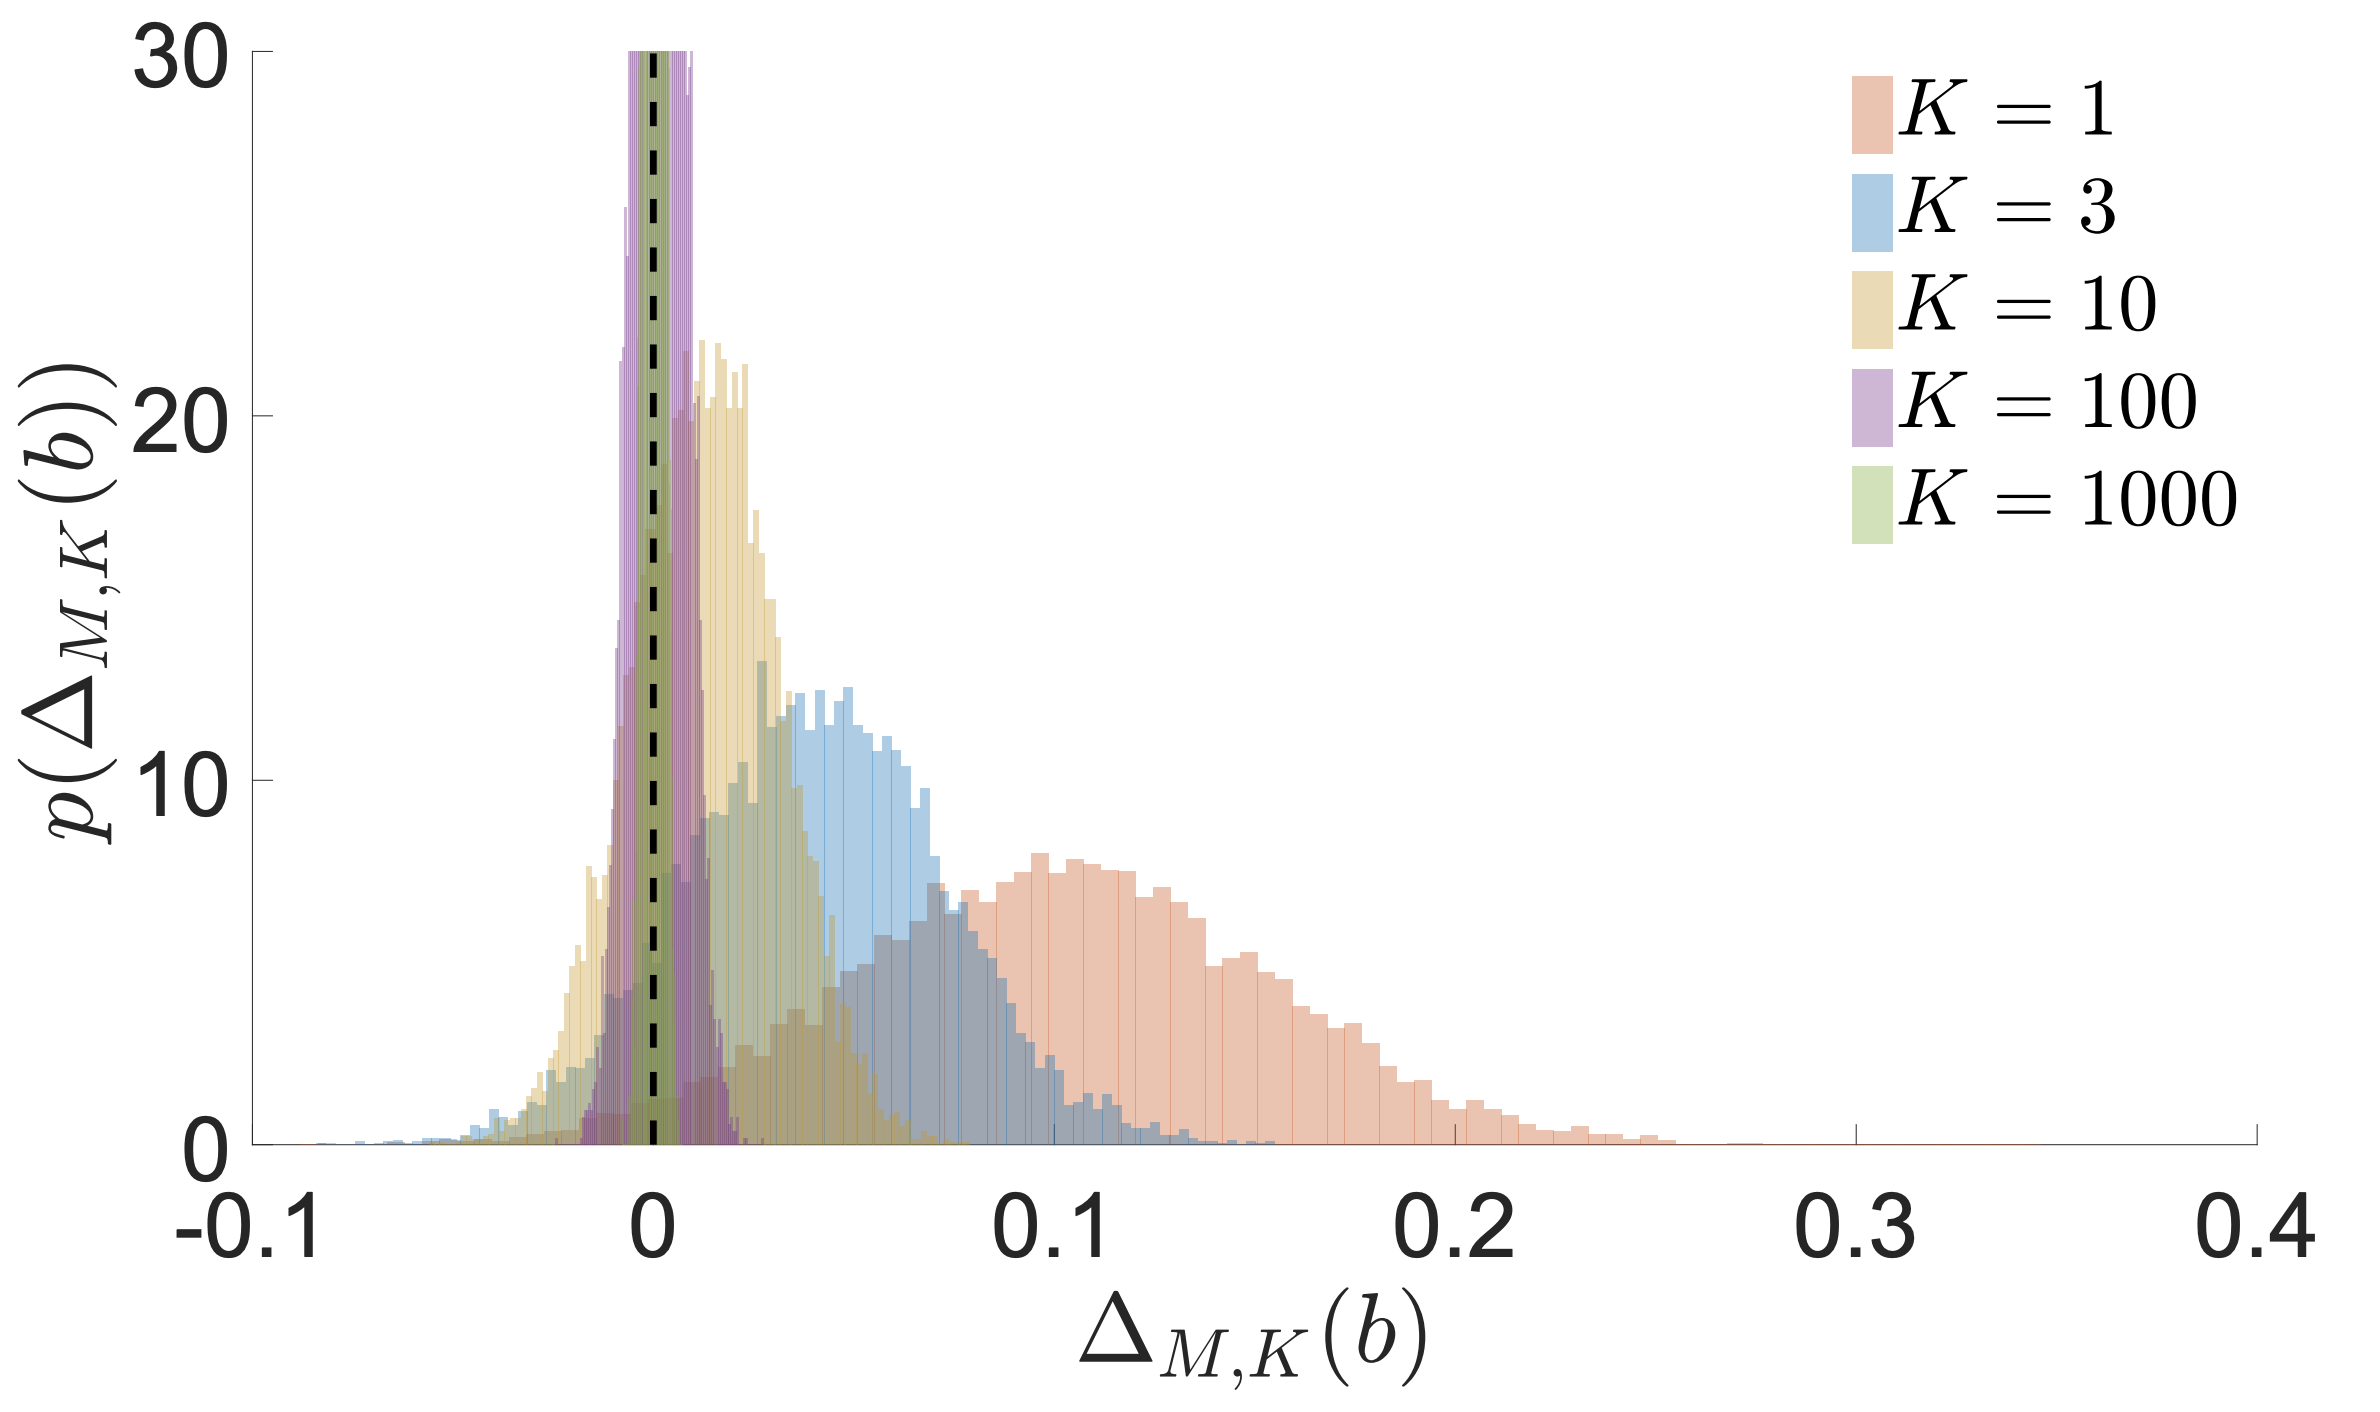
\includegraphics[width=1.\linewidth]{figs/IWAE_SNR_1.png}
			\end{figure}
		\end{minipage}%
		\begin{minipage}[t]{0.5\columnwidth}
			\begin{figure}[h]
				\centering
				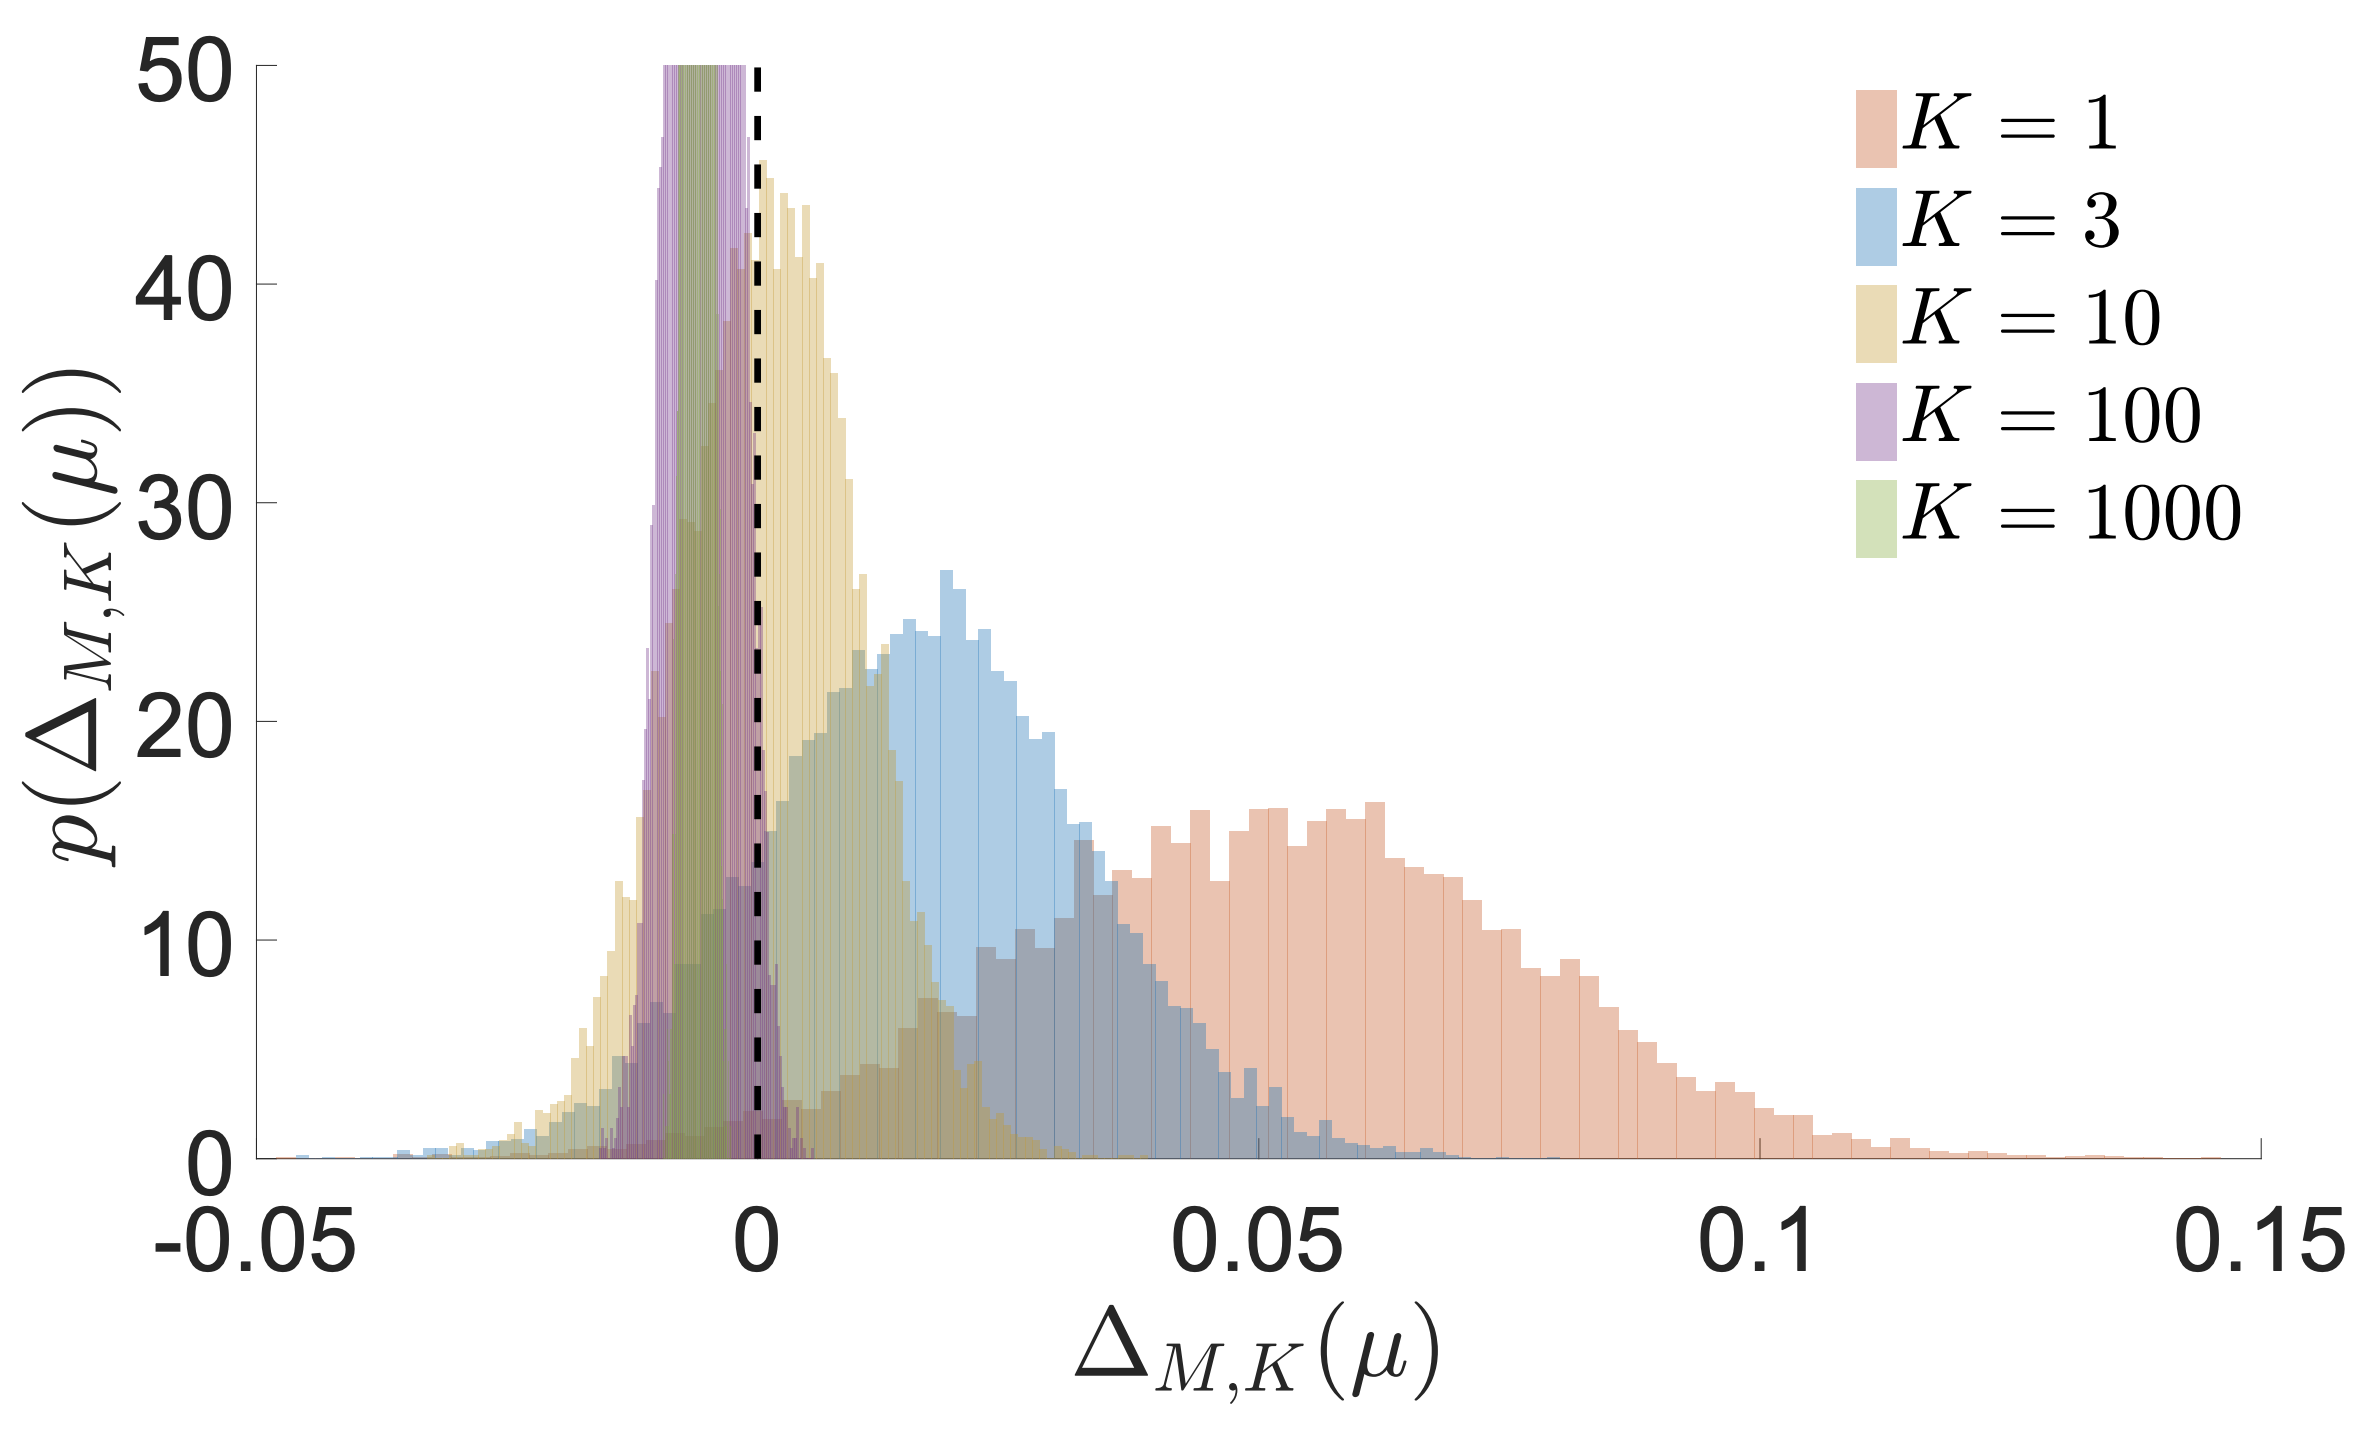
\includegraphics[width=1.\linewidth]{figs/IWAE_SNR_2.png}
			\end{figure}
		\end{minipage}
	\begin{itemize}
		\item IWAE makes the variational bound tighter and extends the class of variational distributions.
		\item Gradient signal becomes really small, training is complicated.
		\item IWAE is very popular technique as a quality measure for VAE models.
	\end{itemize}
	\myfootnotewithlink{https://arxiv.org/abs/1802.04537}{Rainforth T. et al. Tighter variational bounds are not necessarily better, 2018}
\end{frame}
%=======
\begin{frame}{VAE limitations}
	\begin{itemize}
		\item Poor variational posterior distribution (encoder)
		\[
			q(\bz | \bx, \bphi) = \mathcal{N}(\bz| \bmu_{\bphi}(\bx), \bsigma^2_{\bphi}(\bx)).
		\]
		\item Poor prior distribution
		\[
			p(\bz) = \mathcal{N}(0, \mathbf{I}).
		\]
		\item Poor probabilistic model (decoder)
		\[
			p(\bx | \bz, \btheta) = \mathcal{N}(\bx| \bmu_{\btheta}(\bz), \bsigma^2_{\btheta}(\bz)).
		\]
		\item Loose lower bound
		\[
			\log p(\bx | \btheta) - \mathcal{L}(q, \btheta) = (?).
		\]
	\end{itemize}
\end{frame}
%=======
\begin{frame}{ELBO interpretations}
	\[
		\log p(\bx | \btheta) = \cL (\bphi, \btheta) + KL(q(\bz | \bx, \bphi) || p(\bz | \bx, \btheta)) \geq  \cL (\bphi, \btheta).
	\]
	\[
		\cL (\bphi, \btheta) = \int q(\bz | \bx, \bphi) \log \frac{p(\bx, \bz | \btheta)}{q(\bz | \bx, \bphi)} d \bz.
	\]
	\begin{itemize}
	    \item Evidence minus posterior KL
	    \vspace{-0.1cm}
	    \[
	        \mathcal{L}(q, \btheta) = \log p(\bx | \btheta) - KL(q(\bz | \bx, \bphi) || p(\bz | \bx, \btheta)).
	    \]
	    \item Average negative energy plus entropy
	    \vspace{-0.1cm}
	    \begin{align*}
	        \mathcal{L}(q, \btheta) &= \mathbb{E}_{q(\bz | \bx, \bphi)} \left[\log p(\bx, \bz | \btheta) - \log q(\bz | \bx, \bphi)  \right] \\
	        &= \mathbb{E}_{q(\bz | \bx, \bphi)} \log p(\bx, \bz | \btheta) + \mathbb{H} \left[q(\bz | \bx, \bphi) \right].
	    \end{align*}
	    \item Average reconstruction minus KL to prior
	    \vspace{-0.1cm}
	    \begin{align*}
	        \mathcal{L}(q, \btheta) &= \mathbb{E}_{q(\bz | \bx, \bphi)} \left[ \log p(\bx | \bz, \btheta) + \log p(\bz) - \log q(\bz | \bx, \bphi) \right] \\
	        &= \mathbb{E}_{q(\bz | \bx, \bphi)} \log p(\bx | \bz, \btheta) - KL(q(\bz | \bx, \bphi) || p(\bz)).
	    \end{align*}
	\end{itemize}
\end{frame}
%=======
\begin{frame}{ELBO surgery}
	\vspace{-0.3cm}
	\[
	    \frac{1}{n} \sum_{i=1}^n \mathcal{L}_i(q, \btheta) = \frac{1}{n} \sum_{i=1}^n \left[ \mathbb{E}_{q(\bz | \bx_i)} \log p(\bx_i | \bz, \btheta) - KL(q(\bz | \bx_i) || p(\bz)) \right].
	\]
	\vspace{-0.3cm}
	\begin{block}{Theorem}
		\[
		    \frac{1}{n} \sum_{i=1}^n KL(q(\bz | \bx_i) || p(\bz)) = KL(q(\bz) || p(\bz)) + \bbI_{q} [\bx, \bz],
		\]
		\begin{itemize}
			\item $q(\bz) = \frac{1}{n} \sum_{i=1}^n q(\bz | \bx_i)$ -- \textbf{aggregated} posterior distribution.
			\item $\bbI_{q} [\bx, \bz]$ -- mutual information between $\bx$ and $\bz$ under empirical data distribution and distribution $q(\bz | \bx)$.
			\item First term pushes $q(\bz)$ towards the prior $p(\bz)$.
			\item Second term reduces the amount of	information about $\bx$ stored in $\bz$. 
		\end{itemize}
	\end{block}
	\myfootnotewithlink{http://approximateinference.org/accepted/HoffmanJohnson2016.pdf}{Hoffman M. D., Johnson M. J. ELBO surgery: yet another way to carve up the variational evidence lower bound, 2016}
\end{frame}
%=======
\begin{frame}{ELBO surgery}
	\begin{block}{Theorem}
	\[
	    \frac{1}{n} \sum_{i=1}^n KL(q(\bz | \bx_i) || p(\bz)) = KL(q(\bz) || p(\bz)) + \bbI_q [\bx, \bz].
	\]
	\end{block}
	\begin{block}{Proof}
	\vspace{-0.3cm}
	{\footnotesize
	\begin{multline*}
	    \frac{1}{n} \sum_{i=1}^n KL(q(\bz | \bx_i) || p(\bz)) = \frac{1}{n} \sum_{i=1}^n \int q(\bz | \bx_i) \log \frac{q(\bz | \bx_i)}{p(\bz)} d \bz = \\
	    = \frac{1}{n} \sum_{i=1}^n \int q(\bz | \bx_i) \log \frac{q(\bz) q(\bz | \bx_i)}{p(\bz)q(\bz)} d \bz 
	    = \int \frac{1}{n} \sum_{i=1}^n  q(\bz | \bx_i) \log \frac{q(\bz)}{p(\bz)} d \bz + \\ 
	    + \frac{1}{n}\sum_{i=1}^n \int q(\bz | \bx_i) \log \frac{q(\bz | \bx_i)}{q(\bz)} d \bz = 
	     KL (q(\bz) || p(\bz)) + \frac{1}{n}\sum_{i=1}^n KL(q(\bz | \bx_i) || q (\bz))
	\end{multline*}
	}
	\end{block}

	\myfootnotewithlink{http://approximateinference.org/accepted/HoffmanJohnson2016.pdf}{Hoffman M. D., Johnson M. J. ELBO surgery: yet another way to carve up the variational evidence lower bound, 2016}
\end{frame}
%=======
\begin{frame}{ELBO surgery}
	\begin{block}{Theorem}
			\[
			    \frac{1}{n} \sum_{i=1}^n KL(q(\bz | \bx_i) || p(\bz)) = KL(q(\bz) || p(\bz)) + \bbI_{q} [\bx, \bz],
			\]
	\end{block}
	\begin{block}{Proof (continued)}
	\vspace{-0.5cm}
		\[
		    \frac{1}{n} \sum_{i=1}^n KL(q(\bz | \bx_i) || p(\bz_i)) = KL (q(\bz) || p(\bz)) + \frac{1}{n}\sum_{i=1}^n KL(q(\bz | \bx_i) || q (\bz))
		\]
		It could be shown (exercise):
		\[
			\bbI_{q} [\bx, \bz] = \frac{1}{n}\sum_{i=1}^n KL(q(\bz | \bx_i) || q (\bz)) \in [0, \log n].
		\]
	\end{block}

	\myfootnotewithlink{http://approximateinference.org/accepted/HoffmanJohnson2016.pdf}{Hoffman M. D., Johnson M. J. ELBO surgery: yet another way to carve up the variational evidence lower bound, 2016}
\end{frame}
%=======
\begin{frame}{Summary}
	\begin{itemize}
		\item Uniform dequantization is the simplest form of dequantization. 
		\vfill
		\item Variational dequantization is a more natural type that was proposed in Flow++ model.
		\vfill
		\item The IWAE could get the tighter lower bound to the likelihood, but the training of such model becomes more difficult.
		\vfill
		\item The ELBO surgery reveals insights about a prior distribution in VAE. The optimal prior is the aggregated posterior.
	\end{itemize}
\end{frame}

\end{document} 